\section{Introduction}


The original concept for the \CC was to put it at the base in La Serena (\cite[Sec. 9]{LDM-148}),
but there are a number of problems with this:
\begin{itemize}
\item
  Data taken on the summit would have to be transferred to the base, and ingested into a separate butler
\item
  We would have to install, and maintain, a batch processing system at the base (including managing
  the butler registry)
\item
  Some of the functionality provided by the \CC is needed to monitor the survey data quality,
  and it is not clear that the summit-base link is reliable enough to guarantee that the results of this
  analysis will always be available at the summit.  Depending on the definition of `degraded mode' this
  may or may not be a problem
\end{itemize}

Accordingly, we propose that the \CC nodes be moved to the summit, to augment a pre-existing cluster, yagan.
We note that much of the most compute-intensive work during commissioning is expected to be carried out at
USDF (\cite{RTN-021}).
The benefits of this modified topology for the IT group include:
\begin{itemize}
    \item Reduced administration overhead 
    \item Limit security constraints to a single location
    \item Simplifies configuration deployment
    \item Promotes summit independence 
\end{itemize}
The big picture of the current topology is the following:

\begin{figure}
    \centering
    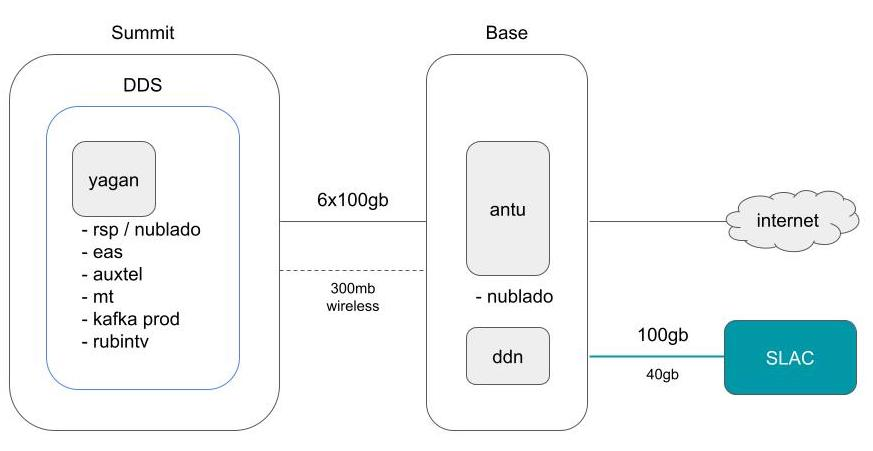
\includegraphics[width=18cm]{images/current_state.jpg}
    \caption{topology}
\end{figure}

\newpage
